% *******************************************************
% SUPPRESS WARNINGS
% *******************************************************
\RequirePackage{silence}
\WarningFilter{scrbook}{Usage of package `titlesec'}
\WarningFilter{titlesec}{Non standard sectioning command detected}

% *******************************************************
% DOCUMENT FRONT MATTER START
% *******************************************************
\documentclass[11pt,twoside,openright,titlepage,
  headinclude,footinclude,BCOR=5mm,
  numbers=noenddot,cleardoublepage=empty,
  tablecaptionabove, dottedtoc,
  bibliography=totoc]{scrreprt}
\usepackage{subfig}
\usepackage[eulerchapternumbers, subfig, beramono, eulermath, pdfspacing]{classicthesis} 
\usepackage{arsclassica}
\usepackage{graphicx}
\usepackage{booktabs}
\usepackage[utf8]{inputenc}
\usepackage[T1]{fontenc}
\usepackage{pdfpages}
\usepackage{titlesec}
\usepackage{titletoc}
\usepackage[norsk,american]{babel}
\usepackage[paperwidth=17cm, paperheight=24cm, margin=2.5cm]{geometry}
\usepackage[cam,a4,center,pdflatex]{crop}

% *******************************************************
% ADDITIONAL PACKAGES
% *******************************************************

% *******************************************************
% REFERENCE PACKAGES
% *******************************************************
  \usepackage[authoryear]{natbib}
  \bibliographystyle{plainnat}

% *******************************************************
% DEFINE VARIABLES
% *******************************************************
\newcommand{\Name}{Raju Rimal}
\newcommand{\Title}{Exploration of Multi-Response Multivariate Methods}
\newcommand{\Location}{\spacedlowsmallcaps{Ås}}
\newcommand{\Year}{2019}
\newcommand{\Month}{april}
\newcommand{\Date}{\Year, \Month}
\newcommand{\docsite}{\url{https://therimalaya.github.com/thesis}}
\newcommand{\Subtitle}{}
\newcommand{\email}{\mail{raju.rimal@nmbu.no}}
\newcommand{\homepage}{\url{https://www.mathatistics.com/}}
\newcommand{\Affiliation}{Biostatistics\\
Dept. of Chemistry, Biotechnology and Food Science\\
Norwegian University of Life Sciences}
\newcommand{\Faculty}{}
\newcommand{\Group}{}
\newcommand{\alttitle}{Utforskning av multi-respons multivariate metoder}

% *******************************************************
% CUSTOMIZATIONS
% *******************************************************
\newcommand{\mail}[1]{\href{mailto:#1}{\texttt{#1}}}
\titlecontents{part}[0pt]{\pagebreak}{}{\Large\MakeTextUppercase}{}
\titleformat{\part}[display]
  {\normalfont\centering\Large}%
  {\thispagestyle{empty}\partname~\MakeTextUppercase{\thepart}}{1em}%
  {\color{Maroon}\spacedallcaps}
\providecommand{\tightlist}{%
  \setlength{\itemsep}{0pt}\setlength{\parskip}{0pt}}
\DeclareTOCStyleEntry[beforeskip=3pt]{tocline}{section}

% *******************************************************
% DOCUMENT BEGIN
% *******************************************************
\begin{document}
\pagenumbering{Roman}
\pagestyle{plain}

% *******************************************************
% Title Front
% *******************************************************
\begin{titlepage}
  \pdfbookmark{Titlepage}{Titlepage}
  \begin{center}
    \large \sffamily
    \bigskip
    {\huge\spacedlowsmallcaps{\Title} \\}
    \bigskip
    {\large{\alttitle}} \\
    \vfill
    {\Large\spacedlowsmallcaps{Doctor of Philosophy (PHD) Thesis}} \\
    \bigskip
    {\Large{\spacedlowsmallcaps\Name}} \\
    \vfill
    {\normalsize \Affiliation}
    \vfill
    {\normalsize \Location, \Year \\}
    \vfill
              \newcommand{\logowidth}{0.6\linewidth}
          
\includegraphics[width=\logowidth]{Logo.pdf} \\
        \vfill
    {\normalsize
      Thesis Number: 1234:56\\
      ISSN:  1234-5678\\
      ISBN:  123-45-678-1234-5\\
    }
  \end{center}
\end{titlepage}

% *******************************************************
% Title Back
% *******************************************************
\thispagestyle{empty}
\hfill \vfill
\noindent
\textit{The goal is to turn data into information, and information into insight.}\\
\spacedlowsmallcaps{- Carly Fiorina, former CEO of Hewlett-Packard}
\vfill
\noindent
{\textbf{Supervisors:}} \\
Professor \textit{Solve Sæbø}\\
Prorector\\
Norwegian University of Life Sciences\\
Ås, Norway\\
\medskip\\
Associate Professor \textit{Trygve Almøy}\\
Dept. of Chemistry, Biotechnology and Food Science\\
Norwegian University of Life Sciences\\
Ås, Norway\\
\medskip\\
\bigskip \\
\noindent
\textit{\Title} \\
{\spacedlowsmallcaps{PhD Thesis, \Date\,\, \textcopyright\, \Name}} \\
\bigskip \\
\noindent{\spacedlowsmallcaps{Website}}: \\
\docsite
\medskip
\noindent{\spacedlowsmallcaps{E-mail}}: \\
\email
\vspace{1cm}
\hrule
\bigskip
\noindent This thesis is prepared with \texttt{ArsClassica} \LaTeX~template with \texttt{pandoc} and r-package \texttt{bookdown}.\\
Source: \url{https://github.com/therimalaya/thesis}
\pagestyle{scrheadings} 

% *******************************************************
% ABSTRACT
% *******************************************************

% *******************************************************
% SUMMARY
% *******************************************************
\begingroup
\pdfbookmark{Summary}{Summary}
\addchap{Summary}
A linear regression model defines a linear relationship between two or
more random variables. The random variables that depend on other random
variables are often called response variables and the independent random
variables are called predictor variables. In most cases not all
variation is relevant for regression, i.e.~only a certain amount of the
variation in the predictors is relevant and only so for a part of the
variation in the response. This leads to a reduction of the linear
regression model where one can imagine a subspace of the space spanned
by the predictor variables that contains all the relevant information
for a subspace of the space spanned by the response variables.

In this thesis we attempt to compare some new methods which are based on
the envelope model and some established methods such as principal
components regression (PCR) and partial least squares regression (PLS).
The comparison tests these methods on their performance of producing
minimum prediction and estimation error while modelling data simulated
with specifically designed properties. For the simulation we have also
created an R-package called \texttt{simrel} with a web interface.

A simulation model for a multi-response multivariate linear model, on
which the simulation tool is based, is discussed in the first paper.
This paper prepares a basic foundation for the simulations with the
concept of reduction of regression models. The second paper discusses
the similarities of the envelope, PCR and PLS population models. This
paper compares the prediction performance of several multivariate
methods using a model with a single response.

The final two papers make an extensive investigation evaluating the
prediction and estimation performance of established (PCR, PLS1 and
PLS2) and newly developed envelope based (Xenv and Senv) methods.
Unsurprisingly the study found that not one method dominates in all
situations, but their performance depend on the properties of the data
they model. However, the envelope based methods have shown remarkable
performance in many cases, both in prediction and estimation. The study
also recommend researchers to use and evaluate the envelope methods.


\KOMAoptions{open=left}
\begin{otherlanguage}{norsk}
\pdfbookmark{Sammendrag}{Sammendrag}
\addchap{Sammendrag}
En lineær regresjonsmodell definerer et lineært forhold mellom to eller
flere tilfeldige variabler. De tilfeldige variablene som er avhengige av
andre tilfeldige variabler, kalles ofte responsvariabler, og de
uavhengige tilfeldige variablene kalles prediktorvariabler. I de fleste
tilfeller er ikke all variasjon relevant for regresjon, dvs. bare en
viss mengde variasjonen i prediktorene er relevante, og bare for en del
av variasjonen i responsen. Dette fører til en reduksjon av den lineære
regresjonsmodellen der man kan forestille seg et underrom av rommet som
spennesut av prediktorvariablene som inneholder all relevant informasjon
for et underrom av rommet spent ut av responsvariablene.

I denne avhandlingenprøver vi å sammenligne noen nye metoder som er
basert på Envelopemodellen og noen etablerte metoder som principal
komponent regresjon (PCR) og partiell minste kvadraters regresjon (PLS).
Sammenligningen tester disse metodene på deres ytelse til å produsere
minimum prediksjon- og estimeringsfeil, mens modelleringsdata simuleres
med spesielt designede egenskaper. For simuleringen har vi også laget en
R-pakke kalt \texttt{simrel} med et webgrensesnitt.

En simuleringsmodell for multirespons, multivariat lineær modell, som
simuleringsverktøyet bygger på, diskuteres i den første artikkelen.
Denne artikkelen utarbeider et grunnleggende fundament for simuleringene
basert på konseptet om reduksjon av regresjonsmodeller. Den andre
artikkelen diskuterer likhetene i Envelope-, PCR- og
PLS-populasjonsmodellene. Denne artikkelen sammenligner
prediksjonsytelsen til flere multivariate metoder ved bruk av en modell
med en enkelt respons.

De to siste artiklene gir en grundig evaluering av prediksjons- og
estimeringsegenskapene til etablerte metoder (PCR, PLS1 og PLS2) og
nyutviklede envelope-baserte metoder (Xenv og Senv). Ikke uventet fant
studien at det ikke finnes en enkelt metode som dominerer i alle
situasjoner, men resultatene deres avhenger av egenskapene til dataene
de modellerer. Imidlertid har envelope-baserte metoder vist
bemerkelsesverdig resultater i mange tilfeller, både når det gjelder
prediksjon og estimering. Studien anbefaler også forskere å bruke og
evaluere envelope-metodene.

\end{otherlanguage}{norsk}
\KOMAoptions{open=right}
\endgroup

% *******************************************************
% ACKNOWLEDGMENT
% *******************************************************
\pdfbookmark{Acknowledgments}{Acknowledgments}
\begingroup
\cleardoublepage
\addchap{Acknowledgment}
First and foremost, I am indebted to my supervisor Solve Sæbø who picked
me up from nowhere and brought me into a scientific community by giving
me a chance to pursue this degree. His inspiration and encouragement
have been an essential element in the course of this journey. I am
grateful to my co-supervisor Trygve Almøy for being a mentor, a friend,
a colleague, and a guardian and guiding and supporting me throughout
this period. He has always been there for me with my frustration and
excitement.

I am forever grateful to my father Narayan Prasad Rimal and mother
Bhagawati Rimal for their continuous support and encouragement. Their
belief in me and push for my education have shined the light in my hard
and easy times. I am also thankful to my dear wife Junali Chhetri who
has inspired me every step of my life and help me to better understand
myself. And of course, a thank goes to my beloved son Nirvan Rimal who
has understood my busy time during this study.

I would also like to thank Professor Inge Helland for his insight,
suggestion and comment on many mathematical problems on various
statistical methods presented in the thesis.

Last, but importantly, my thank goes to the Biostatistics group with
whom I have collected beautiful memories. Thanks to all the members of
the group from past and present who have always made my stay at NMBU
happy, festive and full of joy.

\endgroup

% *******************************************************
% PREFACE
% *******************************************************
\pdfbookmark{Preface}{Preface}
\begingroup
\cleardoublepage
\addchap{Preface}
This thesis is a part of Doctor of Philosophy (PhD) study. The first
part of the thesis constitute a gentle introduction to the objective of
the study and some of its background. This is followed by the summary of
individual research paper on which this thesis is based on. The
discussion section tries to bind the finding from theses papers. The
final chapter will discuss the limitations and future prospect of the
study. The second part contains all the papers attached.

An R-package called \texttt{simrel} is available as part of the first
paper included in this thesis. The package lets users simulated data
from a multi-response linear model. The package can be installed from
R-package repository CRAN or from GitHub. In addition, a web application
that gives users a graphical user interface for the package is also
available from GitHub. All the results and the documentations of the
research can be reproduced from the codes in GitHub repository with
software and packages required installed. In addition, one can use
docker image together with the code for reproducing the thesis together
with all included papers. All related resources are listed in the final
chapter.

\endgroup

% *******************************************************
% INCLUDE ANYTHING BEFORE
% *******************************************************

% *******************************************************
% Contents
% *******************************************************
\cleardoublepage
\phantomsection
\pdfbookmark{\contentsname}{tableofcontents}
\setcounter{tocdepth}{2}
\begingroup 
  \let\clearpage\relax
  \let\cleardoublepage\relax
    \tableofcontents
\endgroup
\markboth{\spacedlowsmallcaps{\contentsname}}
{\spacedlowsmallcaps{\contentsname}} 

\begingroup
\cleardoublepage
\listoftables
\vfill
\let\clearpage\relax
\let\cleardoublepage\relax

\listoffigures
\vfill
\endgroup

\begingroup 
  \let\clearpage\relax
  \let\cleardoublepage\relax
\endgroup

\cleardoublepage

% *******************************************************
% BODY START
% *******************************************************

\pagenumbering{arabic}

\hypertarget{introduction}{%
\chapter{Introduction}\label{introduction}}

Try to be precise on the thesis objective, problem and what achievement does the theses is expected to meet.

\begin{itemize}
\tightlist
\item
  What is the thesis about
\item
  Why is this important
\item
  What will it add to the big picture
\end{itemize}

\begin{figure}[!htb]
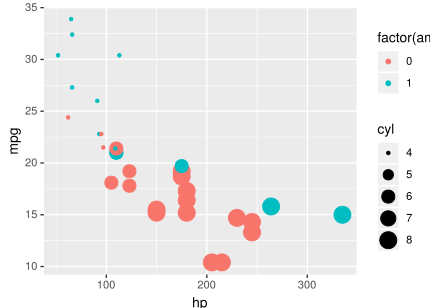
\includegraphics[width=1\linewidth]{Thesis_files/figure-latex/a-test-figure-1} \caption{Test Figure}\label{fig:a-test-figure}
\end{figure}

\begin{table}[t]

\caption{\label{tab:a-test-table}The head of mtcars}
\centering
\begin{tabular}{lrrrrrrr}
\toprule
  & mpg & cyl & disp & hp & drat & wt & qsec\\
\midrule
Mazda RX4 & 21.0 & 6 & 160 & 110 & 3.90 & 2.620 & 16.46\\
Mazda RX4 Wag & 21.0 & 6 & 160 & 110 & 3.90 & 2.875 & 17.02\\
Datsun 710 & 22.8 & 4 & 108 & 93 & 3.85 & 2.320 & 18.61\\
Hornet 4 Drive & 21.4 & 6 & 258 & 110 & 3.08 & 3.215 & 19.44\\
Hornet Sportabout & 18.7 & 8 & 360 & 175 & 3.15 & 3.440 & 17.02\\
\addlinespace
Valiant & 18.1 & 6 & 225 & 105 & 2.76 & 3.460 & 20.22\\
\bottomrule
\end{tabular}
\end{table}

\hypertarget{background}{%
\section{Background}\label{background}}

Write very basic about following topics as an introductory text.

\begin{itemize}
\tightlist
\item
  About reduction of regression model
\item
  Relevant and irrelevant components
\item
  Various study up to this point
\item
  Multi-response model
\item
  Tool for simulation
\end{itemize}

\hypertarget{paper-summary}{%
\chapter{Paper Summary}\label{paper-summary}}

\hypertarget{paper-1-a-tool-for-simulating-multi-response-linear-model-data}{%
\section{Paper 1: A tool for simulating multi-response linear model data}\label{paper-1-a-tool-for-simulating-multi-response-linear-model-data}}

\hypertarget{paper-2-model-and-estimators-for-partial-least-squares-regression}{%
\section{Paper 2: Model and estimators for partial least squares regression}\label{paper-2-model-and-estimators-for-partial-least-squares-regression}}

\hypertarget{paper-3-comparison-of-multi-response-prediction-methods}{%
\section{Paper 3: Comparison of Multi-response Prediction Methods}\label{paper-3-comparison-of-multi-response-prediction-methods}}

\hypertarget{paper-4-comparison-of-multi-response-estimation-methods}{%
\section{Paper 4: Comparison of Multi-response Estimation Methods}\label{paper-4-comparison-of-multi-response-estimation-methods}}

\hypertarget{discussions}{%
\chapter{Discussions}\label{discussions}}

\hypertarget{conclusion-and-future-perspective}{%
\chapter{Conclusion and Future Perspective}\label{conclusion-and-future-perspective}}

% *******************************************************
% BIBLIOGRAPHY START
% *******************************************************
  \renewcommand\refname{References}
 % has-chapters
 % biblio-title
  \bibliography{References.bib}
 % bibliography
 % natbib

 % biblatex

\nocite{*}

% *******************************************************
% PAPER START
% *******************************************************
\appendix

% *******************************************************
% ANYTHING EXTRA
% *******************************************************

\end{document}

%%% Local Variables:
%%% mode: latex
%%% TeX-master: t
%%% End:
